	\begin{figure}[h]
	\centering
		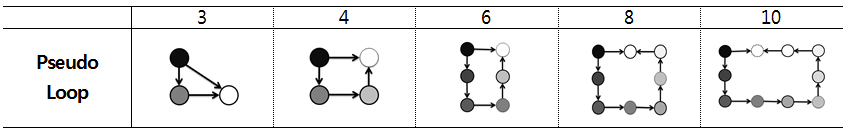
\includegraphics[height=50pt]{Topologies_PseudoLoop}
		\caption{Bayesian Network Topologies : Pseudo Loop}
	\end{figure}	

	% Pseudo Loop은, 우선 line 형태를 그린 뒤, 최상의 부모 node가 맨 마지막 자식 node에 종속되는 arc가 추가된 형태이다. 사실 loop는 아니지만, 얼핏 보면 loop처럼 보인다. (사실, 정말 loop가 만들어지면 더 이상 Bayesian Network가 아니다.)
	Pseudo Loop, after first drew a line form, is the best form of arc has been added to the parent node is dependent on the very last child node. Actually loop does not have, it looks like a loop at first glance. (In fact, actually when loop is created, no longer Bayesian Network is not it.)

\begin{figure}[!bhp]
	\centering
		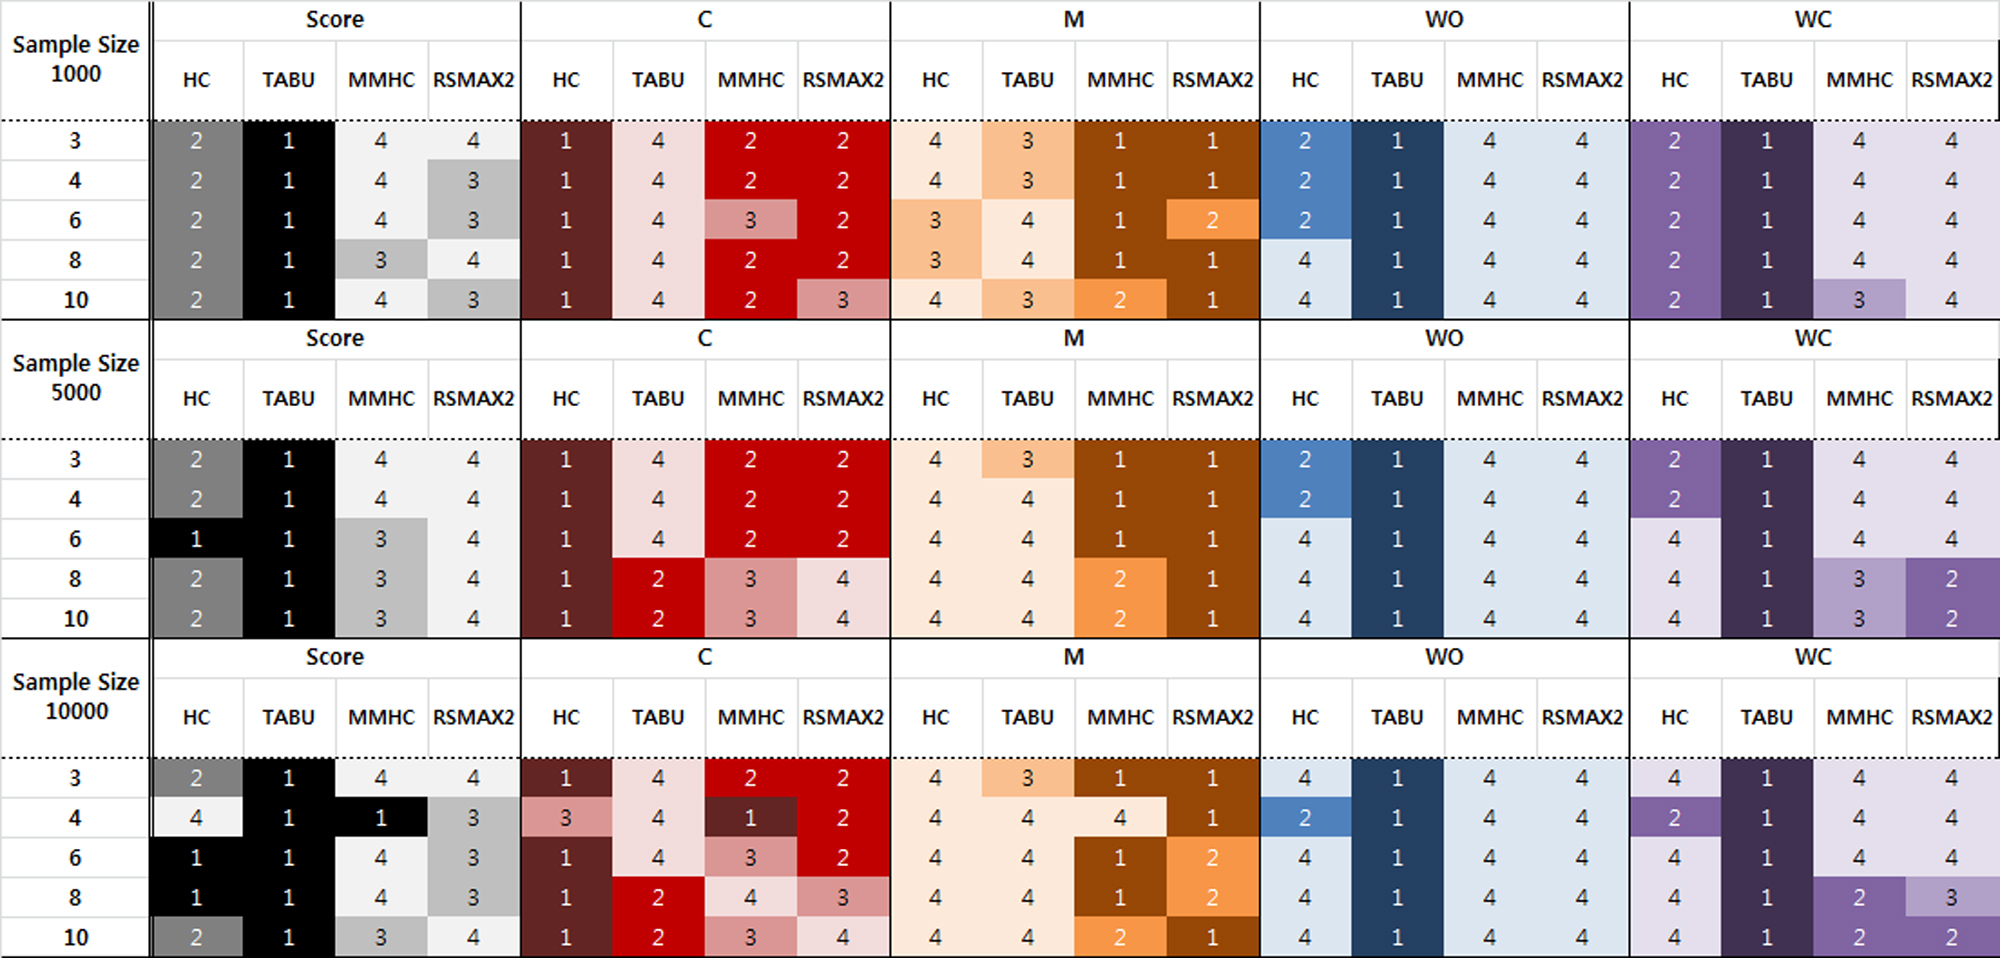
\includegraphics[height=170pt]{Result_PseudoLoop}
		\caption{Summary for Comparison via Pseudo Loop}
	\end{figure}	

% Score 기준으로 비교했을 때는 TABU search가 좋은 성능을 보여주었지만, 목표 네트워크와 학습 네트워크를 비교했을 경우, 상대적으로 Hill-climbing이 line 형태에서 좋은 성능을 보여주었다.
Although TABU search when compared on the basis of exhibited good performance Score, when compared to the network and learning network objectives, relatively Hill-climbing showed good performance in the line form.

% sample size가 1000개일 때는 TABU search의 C의 개수가 개선되지 못했지만, sample size가 커지면 node 개수가 많을 때 C의 개수가 크게 향상되는 모습을 보여주었다. 특히 sample size 증가에 따른 M, WO, WC의 개수 감소가 두드러졌다. 그럼에도 불구하고 Hill-climbing의 성능에 미치지는 못하였다.
If the sample size is 1000 exists, the number of C of TABU search has not been improved, I shows how the number of C when sample size is often node number becomes larger is greatly improved. In particular M with increasing sample size, WO, the reduction in the number of WC was noticeable. And yet, did not give the performance of Hill-climbing.

% 모든 알고리즘이,Sample size가 커짐에 따라 WO, WC 개수가 크게 줄어드는 모습이 나타났다.
All algorithms, WO as Sample size increases, how the number of WC is greatly reduced revealed.
	
	\begin{figure}[p]
	\centering
		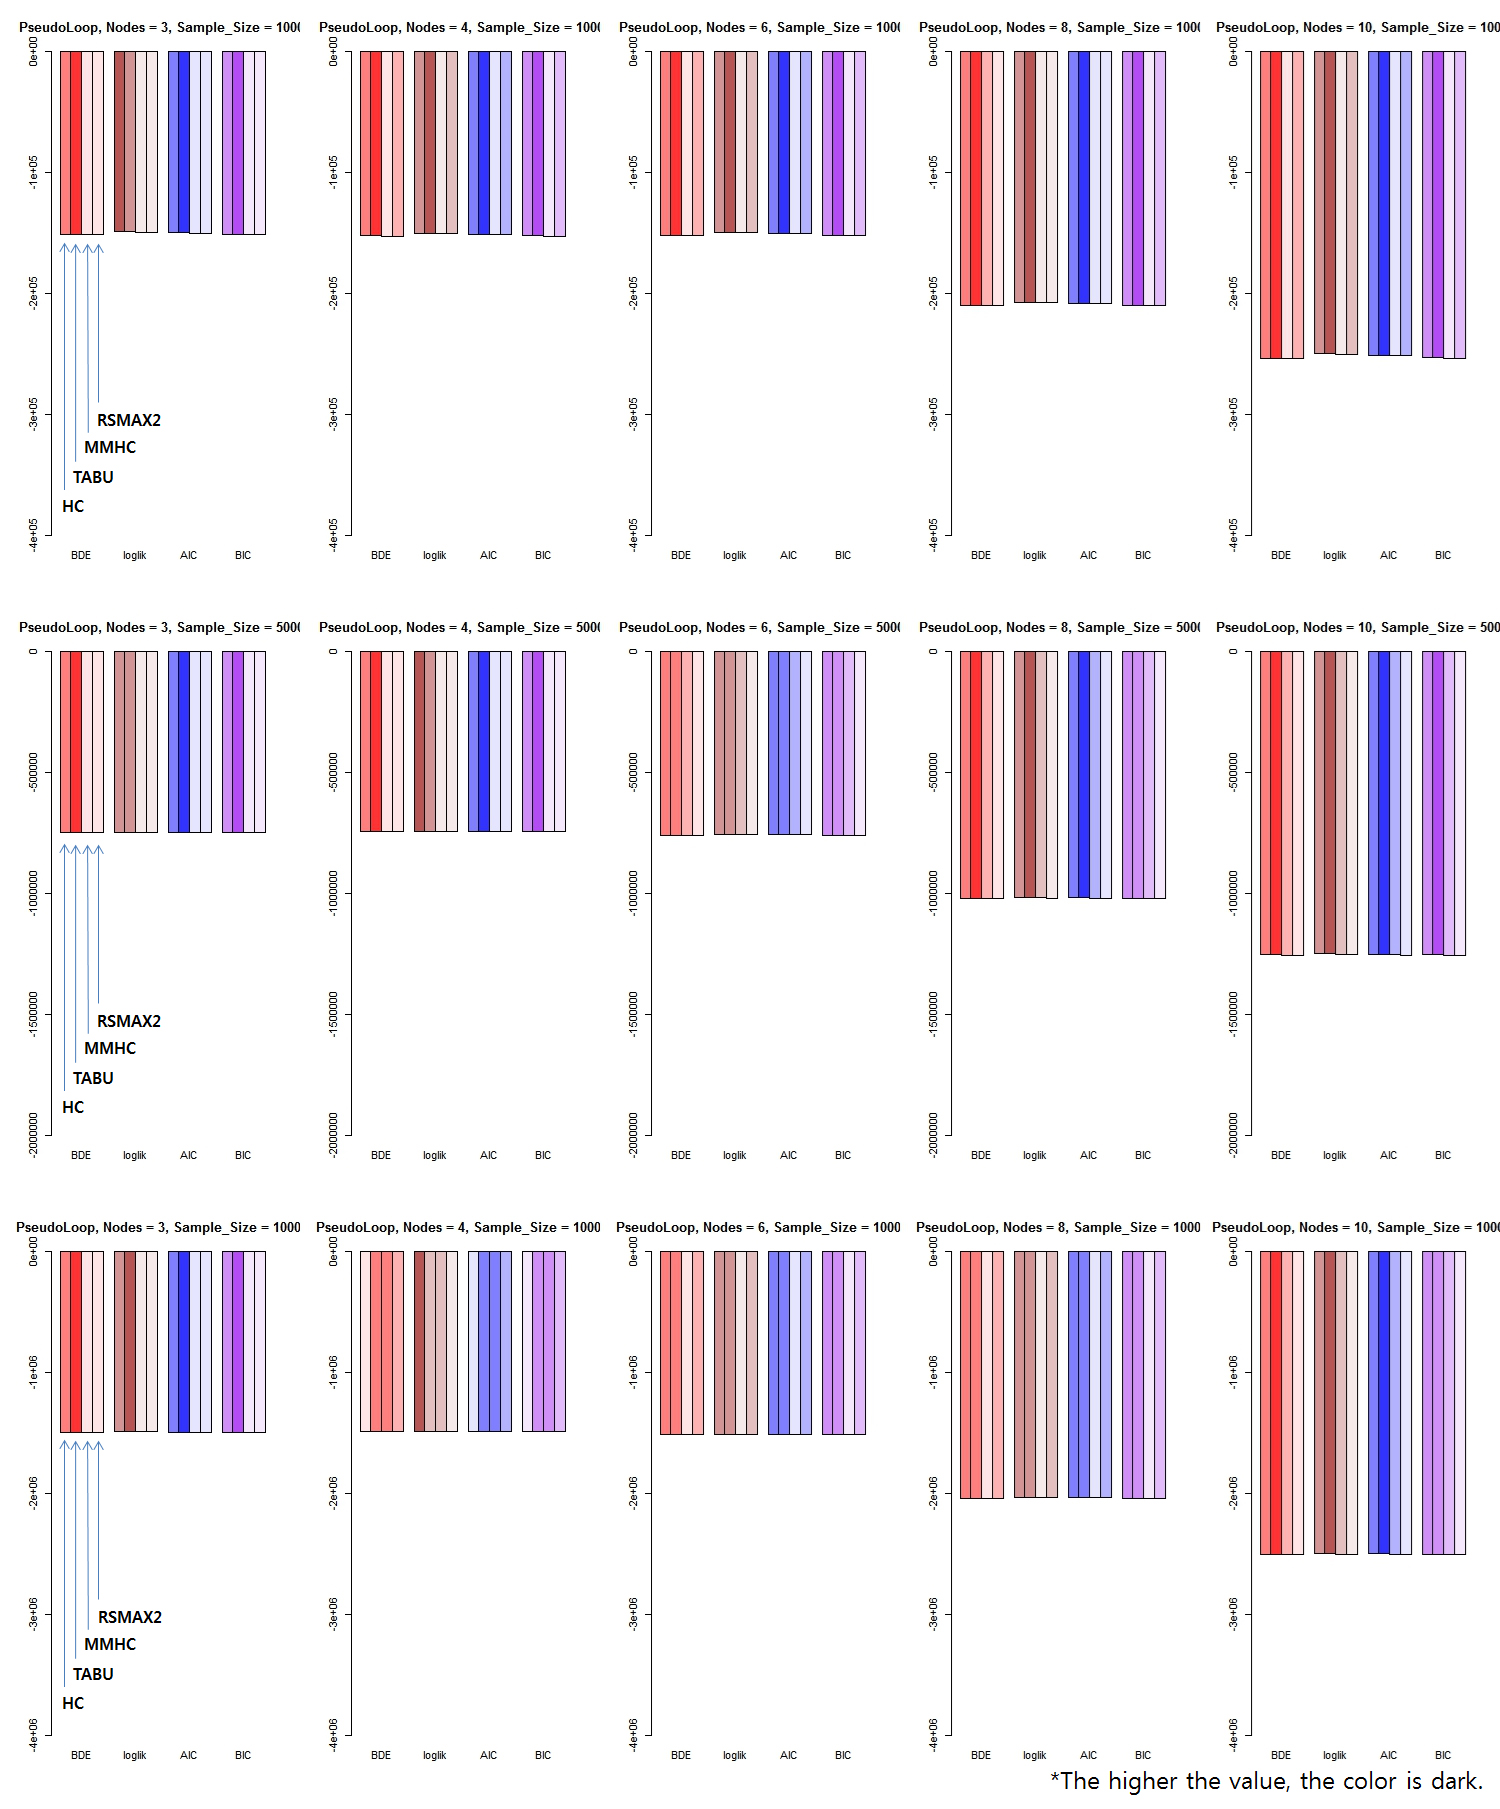
\includegraphics[height=500pt]{04_PseudoLoop_Score}
		\caption{Comparison of scores via Pseudo Loop}
	\end{figure}	

	\begin{figure}[p]
	\centering
		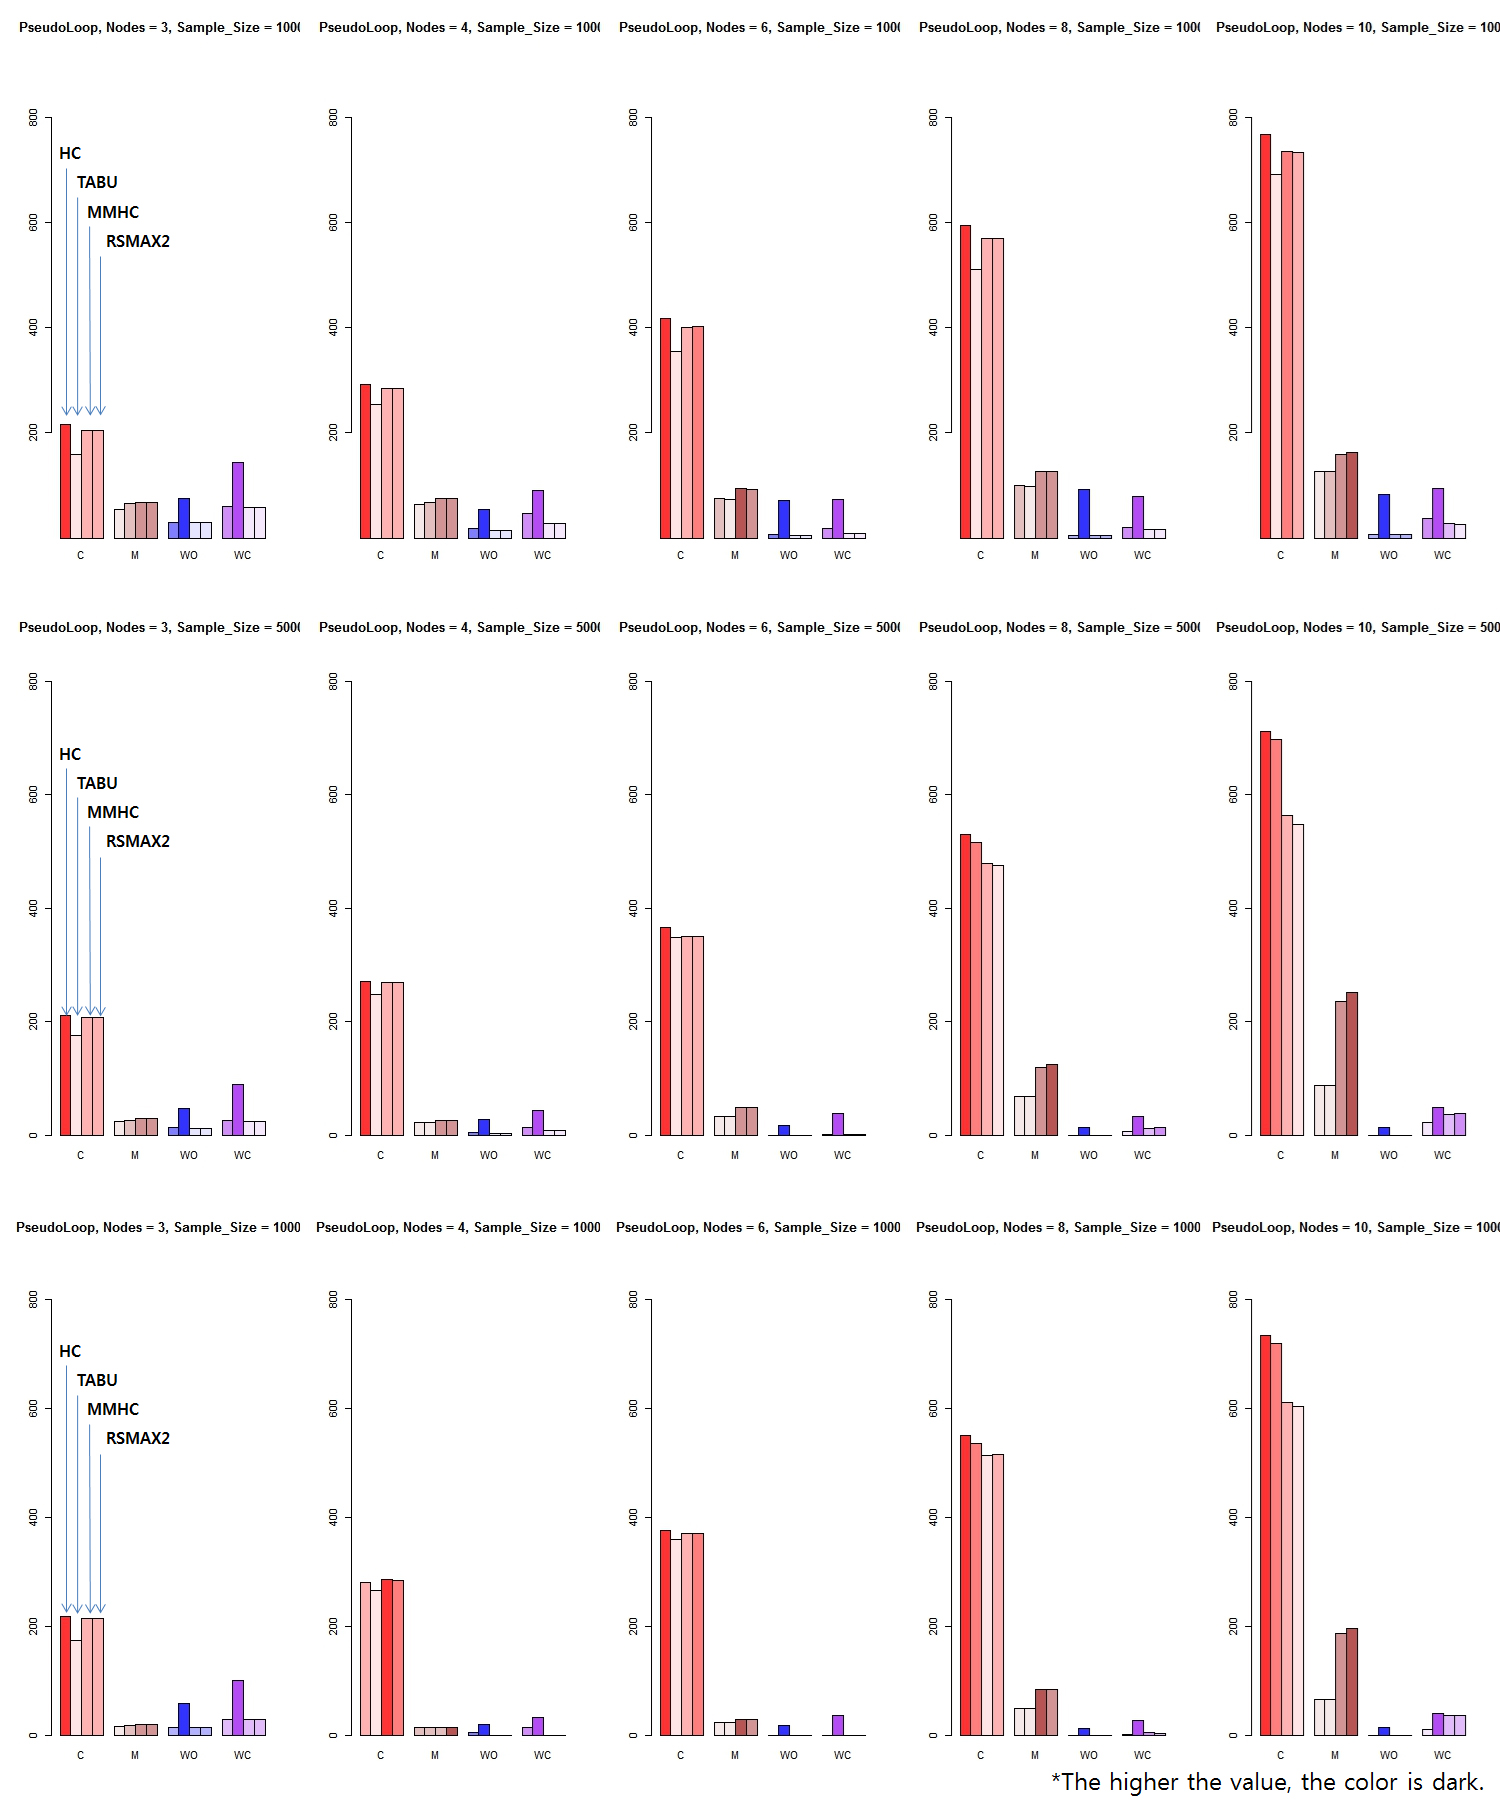
\includegraphics[height=500pt]{04_PseudoLoop_Arcs}
		\caption{Comparison of correct arcs via Pseudo Loop}
	\end{figure}	
